\documentclass[12pt]{article}
\usepackage{amsmath}
\usepackage{amsfonts}
\usepackage[pdftex]{graphicx}
\usepackage{float}

\begin{document}
\noindent \textbf{Daniel Alabi} \\
\textbf{Cody Wang}
\hfill
\textbf{CS 324}\\
\line(1, 0){450} 

\subsection*{Regularized SVD}

In class, we talked about the iterative SVD technique described in the book.
We also talked briefly about how to avoid overfitting; one way to avoid
overfitting is to use regularization [1]. \\

\noindent For the netflix prize competition, Simon Funk implemented a regularized 
iterative SVD technique to predict movie ratings for users [2]. The goal of our
project was to implement a regularized iterative SVD technique, similar
to Simon Funk's. After Simon Funk wrote the article describing his
SVD technique(s), a lot of other data scientists and researchers
have tried to implement his approach. As a result, there is no homogenous
regularized SVD technique. One thing that most of these techniques (including
Simon Funk's) have in common is that they make use of a stochastic 
gradient descent technique to minimize the RMSE [3, 4]. Stochastic gradient 
descent is basically an iterative way to find a local minima of a 
function [5]. In our case, the function to be minimized is the RMSE.

\subsubsection*{Training the U, V matrices}
The crux of the regularized SVD technique we implemented lies in how
the U, V matrices are trained. Recall that, we are trying to ``approximate''
the utility matrix $M$ with two matrices such that
\begin{equation*}
  M \approx U * V^T
\end{equation*}
Note that the singular values of the decomposition have been submerged into
both $U$ and $V^T$. Also, in the algorithm we implemented, instead of 
explicitly storing $V^T$, we store $V$ to make the training step more
seamless. \\

\noindent Training of the $U$ and $V^T$ matrices occurs exactly $r$ times. $r$ is the
rank of the matrix $U*V^T$, or equivalently the number of columns in
$U$, or the number of rows in $V^T$. For each $k$ in $[0, r-1]$, we
call a \textbf{train(k)} method repeatedly (for potentially 
\textbf{maxepochs} times) until the train error, obtained during training
doesn't improve by much ($<$ minimprov). The \textbf{train(k)} method
goes through the entire dataset and for each rating calculates the current
error for the particular user, \textbf{uid}, and movie, \textbf{mid}.
Last, it trains the $k$th column of the user row in $U$ against the
$k$th column of the movie row in $V$ (or equivalently, the $k$th row
of the movie column in $V^T$). It uses the following code:

\begin{figure}[H]
\centering
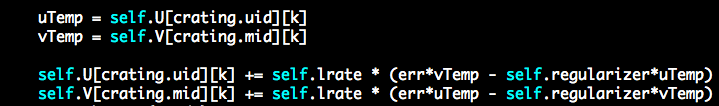
\includegraphics[width=0.90\textwidth]{graphs/trainkcode}
\end{figure}

\noindent This is basically the stochastic gradient descent part of the algorithm
to minimize the RMSE while regularizing to prevent overfitting. 
See [2] for more details. \\

\noindent As the number of epochs progress (for a particular $k$), the RMSE always decreases.\\

\noindent The rank we used ($r$ in our program) was based on 
experiments performed in the next section. Theoretically, $r$ corresponds
to the number of distinct features in the dataset. 


\subsubsection*{Varying the Parameters}

In order to explore the effectiveness of the regularized SVD technique and find
the optimal efficiency for the algorithm, we ran various tests to analyze how the
RMSE and the running time is correlated with three different parameters: the
rank of the matrix ($r$), the learning rate ($lr$), and the regularzier 
($reg$).\\

\noindent We used the 100k and 1M datasets obtained from MovieLens [6] to perform our analyses.
We first set the default values of the $r$, $lr$, and $reg$ to be 10, 0.035, and 0.05,
respectively, which were the values that produced more efficient and accurate
results based on the preliminary trial runs. We then controlled two of the three
parameters while varying one to explore its effect on RMSE and running time of
the algorithm.\\

\noindent For the 100k dataset, we plotted RMSE and running time of both the training dataset
and the test dataset against $r\in$[0, 1, 2,..., 50], $lr\in$[0.005, 0.01, 0.015,..., 0.25], 
and $reg\in[0.001, 0.002, 0.003,..., 0.05]$.\\

\noindent For the 1M dataset, we plotted RMSE and running time of training dataset 
against r$\in$[10, 11, 12,..., 30], lr$\in$[0.005, 0.01, 0.015,..., 0.1], and
reg$\in$[0.001, 0.002, 0.003,..., 0.02].\\

\noindent Figure 1-3 show the relationship between the running time and the three parameters
for the 100k dataset. Running time is the sum of both the running time for the training and
the test datasets. \\

\noindent Figure 1 indicates that the running time is positively correlated
with the matrix rank. Figure 2 indicates that the there is no significant relationship between
running time and the learning rate, but the running time generally increases when $lr\geq$0.15.
Figure 3 shows that there is no significant relationship between running time and
the regularizer.

\begin{figure}[H]
\centering
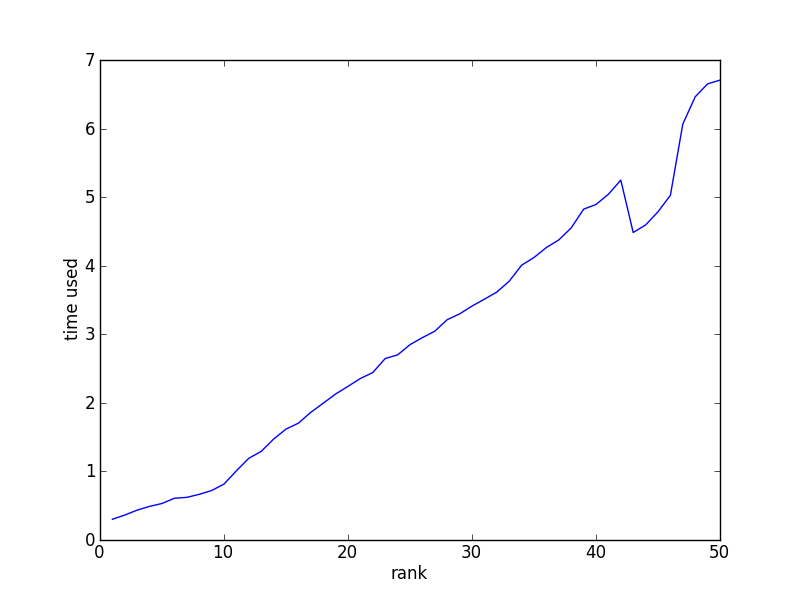
\includegraphics[width=0.60\textwidth]{graphs/smalltimerank.png}
\caption{Relationship between running time and matrix rank for 100k dataset}
\end{figure}

\begin{figure}[H]
\centering
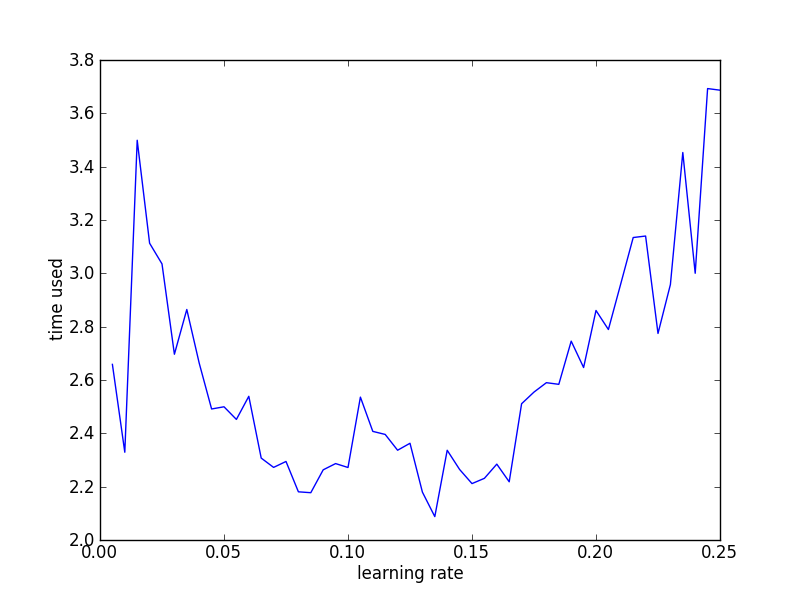
\includegraphics[width=0.60\textwidth]{graphs/smalltimelr.png}
\caption{Relationship between running time and learning rate for 100k dataset}
\end{figure}

\begin{figure}[H]
\centering
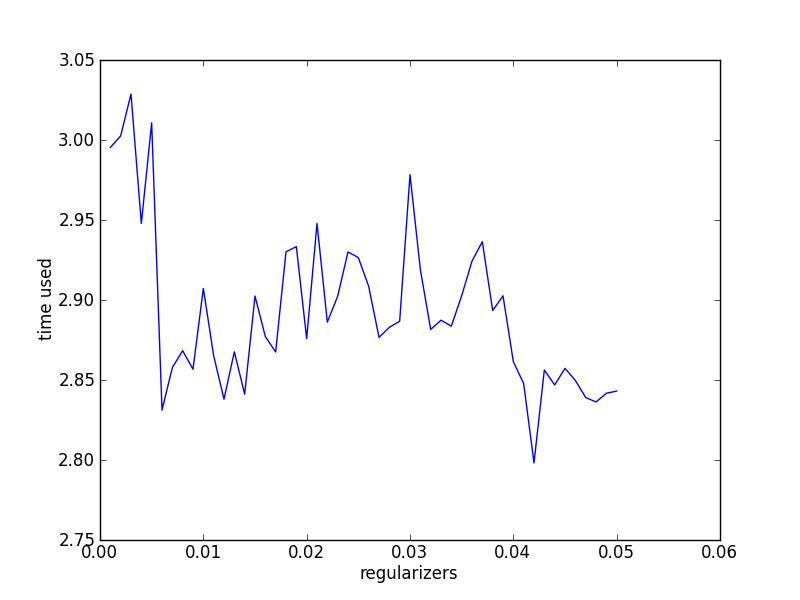
\includegraphics[width=0.60\textwidth]{graphs/smalltimereg.png}
\caption{Relationship between running time and regularizer for 100k dataset}
\end{figure}

\noindent Figure 4-6 show the relationship between the RMSE and the three parameters
for the 100k dataset. Blue dotted lines and red dashed lines represent the RMSE for
the test and the training datasets, respectively.\\

\noindent Figure 4 indicates that the RMSE is generally negatively correlated
with the matrix rank. Figure 5 indicates that the there is a positive correlation
between the RMSE and the learning rate. Figure 6 shows that there is no significant 
relationship between running time and the regularizer for the training dataset. However,
for the test dataset, there is a trend that as regularizer increases, the RMSE increases.

\begin{figure}[H]
\centering
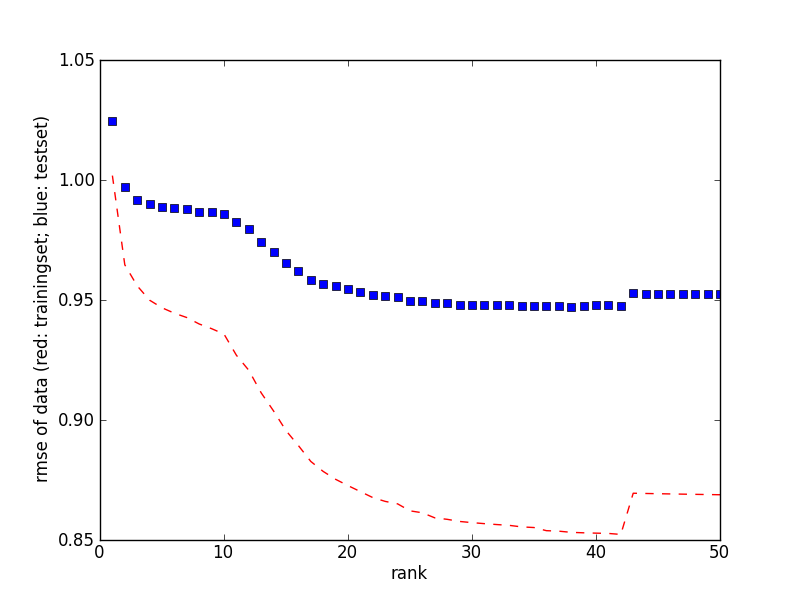
\includegraphics[width=0.60\textwidth]{graphs/smallrmserank.png}
\caption{Relationship between RMSE and matrix rank for 100k dataset}
\end{figure}

\begin{figure}[H]
\centering
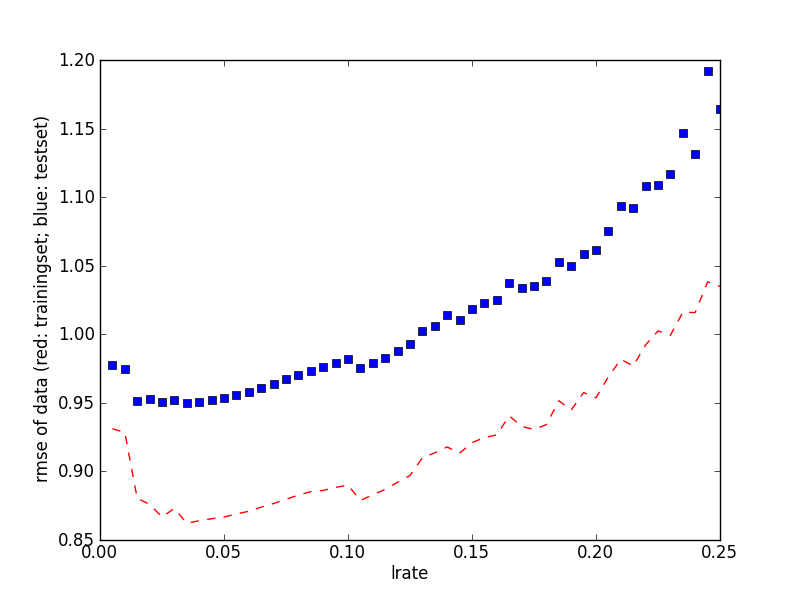
\includegraphics[width=0.60\textwidth]{graphs/smallrmselr.png}
\caption{Relationship between RMSE and learning rate for 100k dataset}
\end{figure}

\begin{figure}[H]
\centering
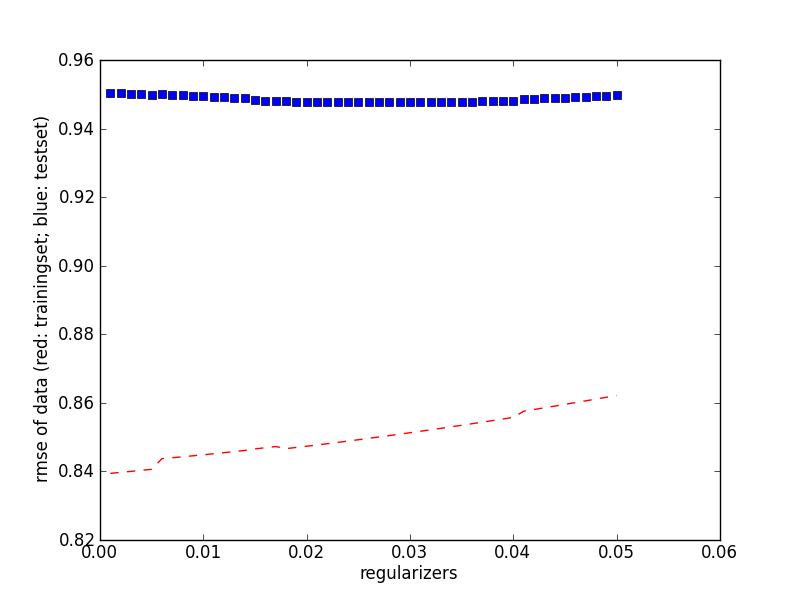
\includegraphics[width=0.60\textwidth]{graphs/smallrmsereg.png}
\caption{Relationship between RMSE and regularizer for 100k dataset}
\end{figure}

\noindent Figure 7-9 show the relationship between the running time and the three parameters
for the 1M dataset.\\

\noindent Figure 7 indicates a positive correlation between the running time
and the matrix rank. Figure 8 indicates that when $lr\leq$0.02, time decreases
as $lr$ increases, but there is no significant relationship between the two after that point.
Figure 9 shows that running time is generally negatively correlated with the regularizer.

\begin{figure}[H]
\centering
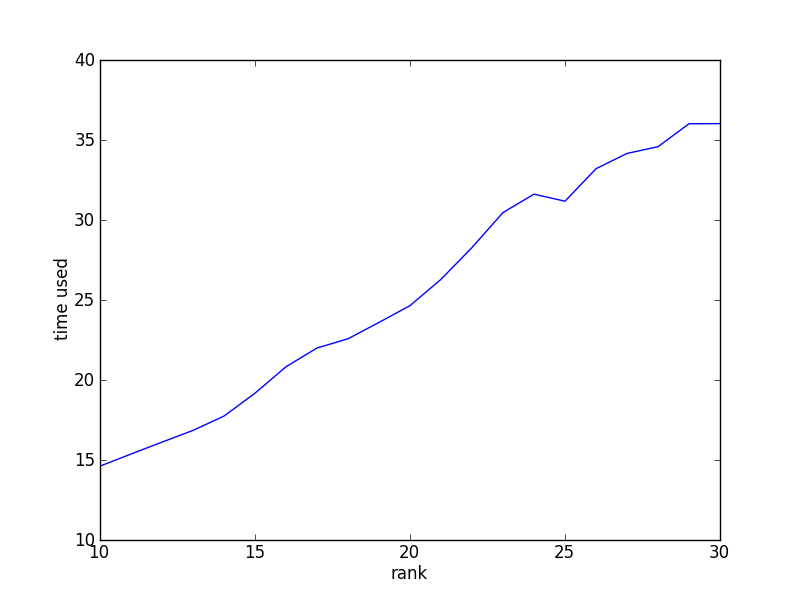
\includegraphics[width=0.60\textwidth]{graphs/bigtimerank.png}
\caption{Relationship between running time and matrix rank for 1M dataset}
\end{figure}

\begin{figure}[H]
\centering
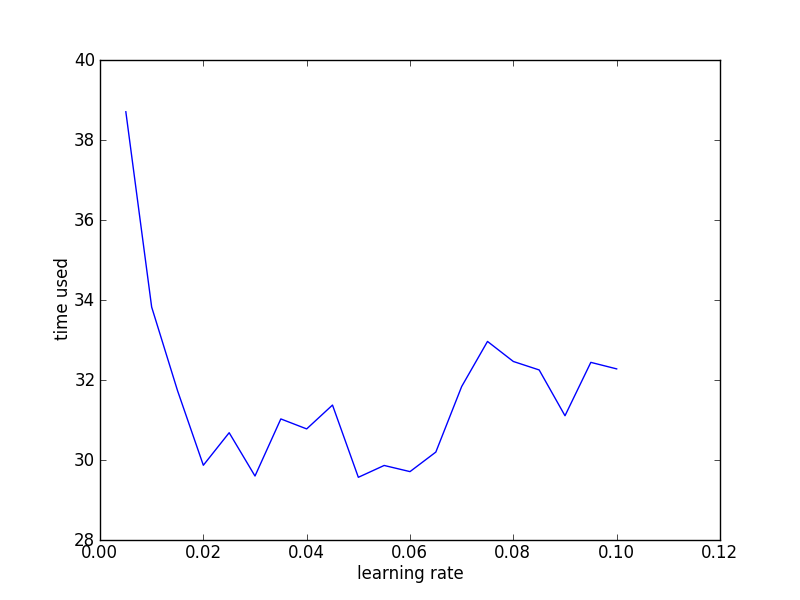
\includegraphics[width=0.60\textwidth]{graphs/bigtimelr.png}
\caption{Relationship between running time and learning rate for 1M dataset}
\end{figure}

\begin{figure}[H]
\centering
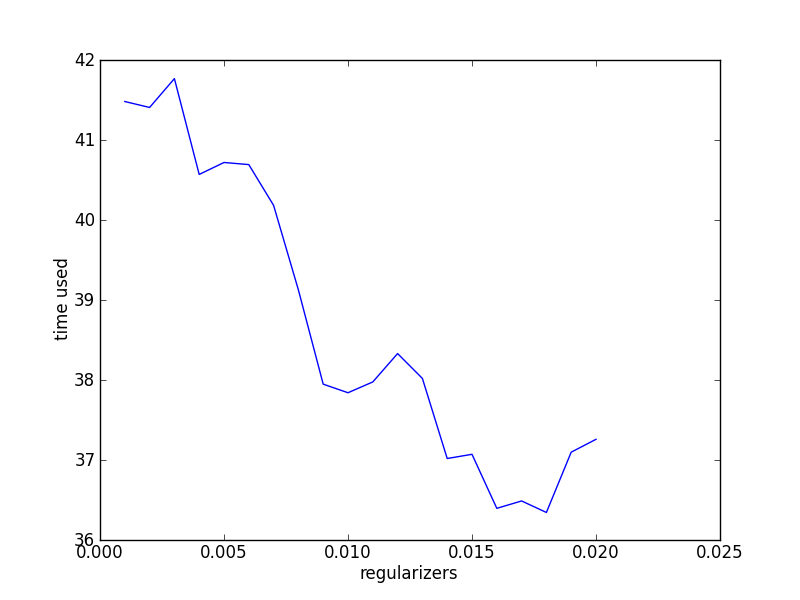
\includegraphics[width=0.60\textwidth]{graphs/bigtimereg.png}
\caption{Relationship between running time and regularizer for 1M dataset}
\end{figure}

\noindent Figure 10-12 show the relationship between the RMSE and the three parameters
for the 1M dataset. \\

\noindent Figure 10 indicates that the RMSE is negatively correlated
with the matrix rank. Figure 11 indicates that the there is a positive correlation
between the RMSE and the learning rate after $lr\geq$0.05. Figure 12 shows that there is a positive correlation between the RMSE and the regularizer.

\begin{figure}[H]
\centering
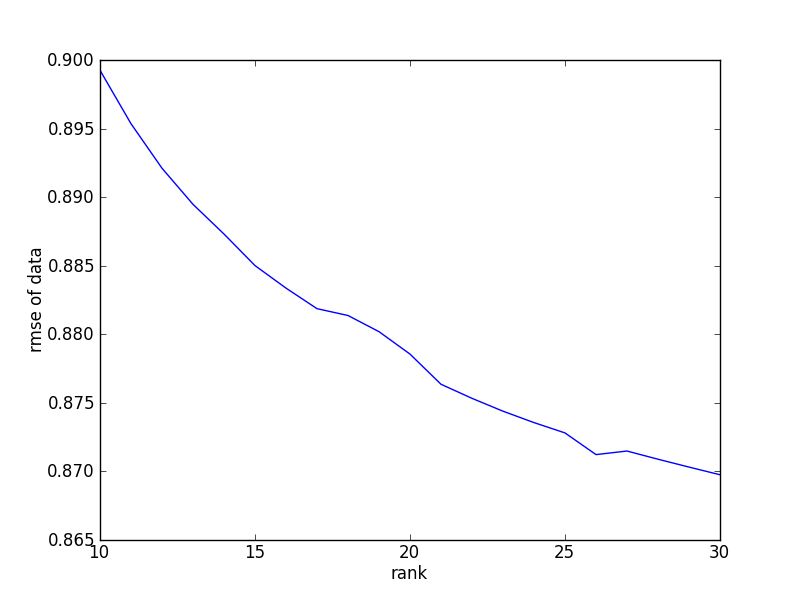
\includegraphics[width=0.60\textwidth]{graphs/bigrmserank.png}
\caption{Relationship between RMSE and matrix rank for 1M dataset}
\end{figure}

\begin{figure}[H]
\centering
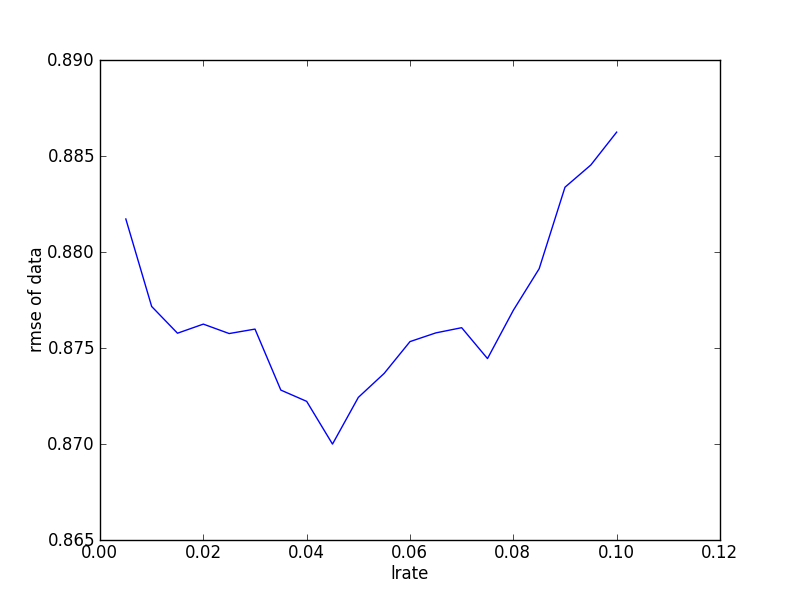
\includegraphics[width=0.60\textwidth]{graphs/bigrmselr.png}
\caption{Relationship between RMSE and learning rate for 1M dataset}
\end{figure}

\begin{figure}[H]
\centering
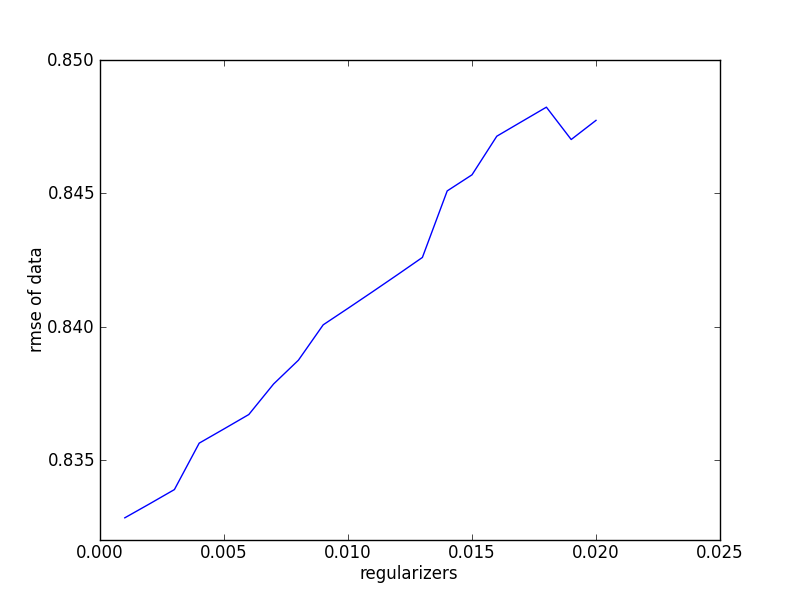
\includegraphics[width=0.60\textwidth]{graphs/bigrmsereg.png}
\caption{Relationship between RMSE and regularizer for 1M dataset}
\end{figure}

\noindent Based on the analyses above, we conclude that:
\begin{enumerate}
  \item Running time of the algorithm is positively correlated with the matrix rank, and has no significant relationship with the learning rate or the regularizer. These results can be explained by the way we implemented the algorithm: since we used $k$ iterations during gradient descent, the running time should be dependent largely on the rank of the matrix.
  \item RMSE is negatively correlated with the matrix rank, and has no significant relationship with the learning rate or the regularizer. However, there exist the trends that as learning rate and the regularizer increase, the RMSE increases. This is especially true for larger datasets.
\end{enumerate}

\subsubsection*{Control Experiments}

In order to explore the advantage of the regularized SVD over 
collaborative-filtering techniques and the normal SVD technique
we introduced in class, we implemented normal SVD using scipy, and
applied both normal SVD and collaborative-filtering (implemented for the
last assignment) on the same datasets as control experiments. We then
compared the results of these controlled experiments against results from 
regularized SVD experiments in the previous section.\\

\noindent For collaborative filtering techniques (item-based and user-based), we set our threshold for nearest neighbor to be 10, and the number of nearest neighbor to be 25.\\

\noindent For normal SVD technique, we kept 20\% of the energy of the diagonal matrix.\\

\noindent For regularized SVD technique, we optimized both RMSE and running time by choosing matrix rank=30, learning rate=0.035, and regularizer=0.01.\\

\noindent We then compared the RMSE and running time of the the four different approaches applied to the 100k test dataset. The results are shown in Table 1 below.

\begin{table}[H]
\caption{RMSE and running time of four recommendations approaches}
$      $
\centering
\begin{tabular}{c c c c c}
\hline\hline
Methods & User-based & Item-based & Normal SVD & Regularized SVD \\ [0.5ex]
\hline
Running Time & 20.303 & 30.444 & 17.099 & 4.137 \\
RMSE (Test) & 0.988 & 0.992 & 1.037 & 0.951 \\ [1ex]
\hline
\end{tabular}
\end{table}

\noindent Based on the table above, we found that the regularized SVD appraoch has both the shortest running time and the lowest RMSE. Although we ran normal SVD with Python instead of pypy, we can still observe that it performs worse than regularized SVD in terms of RMSE. Therefore, we conclude that regularized SVD is the optimal approach among the four.


\subsubsection*{Future Improvements}
\begin{enumerate}
\item Using a cache, just as Simon Funk did, to speed up dot product 
calculations during training.
\item Find a more efficient way to normalize ratings 
for each user.
We tried normalizing. It made our code run slower but made very
little improvement to the RMSE. 
\end{enumerate}

\subsubsection*{References}
\begin{enumerate}
  \item http://en.wikipedia.org/wiki/Regularization\_(mathematics)
  \item http://sifter.org/~simon/Journal/20061211.html
  \item http://www.timelydevelopment.com/demos/NetflixPrize.aspx
  \item http://alias-i.com/lingpipe/docs/api/com/aliasi/matrix/SvdMatrix.html
  \item http://en.wikipedia.org/wiki/Stochastic\_gradient\_descent
  \item http://www.grouplens.org/node/73
\end{enumerate}

\end{document}
